\documentclass[11pt]{article}

\usepackage[review]{acl}

\usepackage{times}
\usepackage{latexsym}
\usepackage[T1]{fontenc}
\usepackage[utf8]{inputenc}
\usepackage{microtype}
\usepackage{inconsolata}
\usepackage{graphicx}
\usepackage{booktabs}
\usepackage{amsmath}
\usepackage{amssymb}

\title{STEM Agent: A Self-Adapting, Tool-Enabled, Extensible Architecture\\
for Multi-Protocol AI Agent Systems in Production}

\author{Anonymous Submission}

\begin{document}
\maketitle

\begin{abstract}
Production AI agent systems increasingly suffer from \emph{architectural lock-in}: early commitment to a single protocol, a fixed tool-integration path, and a static user model makes deployed agents hard to retarget. We describe \textbf{STEM Agent} (Self-adapting, Tool-enabled, Extensible, Multi-agent), an enterprise architecture that unifies five protocols---A2A, AG-UI, A2UI, UCP, and AP2 (the first two published specifications, A2UI extending a community draft, UCP/AP2 first-draft internal designs that fill commerce gaps and have not undergone external security review)---behind a single gateway, isolates domain knowledge behind the Model Context Protocol (MCP), and adapts per-user behavior via a Caller Profiler spanning 21 dimensions. Recurring patterns \emph{crystallize} into reusable skills through a lifecycle managed by a Skills Manager consuming outputs of an ATLAS memory subsystem. We report operational lessons from six months of internal deployment ($\sim$200 weekly users, four production use cases) and ship five industry-aligned persona templates (SRE, finance, AI research, healthcare, legal)---including regulated personas enforcing HIPAA-style PHI guardrails and privileged-communication boundaries through a typed \texttt{forbiddenTopics} contract. We discuss horizontal scaling via externalized state, an opt-in Enterprise Ops surface (RBAC, SIEM audit, CSP/HSTS headers, Prometheus \texttt{/metrics}, PII redaction), pluggable IAM (JWT/OAuth2/SAML/API-Key), and production deployment artifacts (multi-stage non-root Dockerfile, Kubernetes manifests). All hardening controls default off; enabling them is a per-flag decision mirroring deployment-team security-review concerns.
\end{abstract}

\section{Introduction}
\label{sec:intro}

Teams deploying LLM-based agents inside a large enterprise quickly discover that the hard problems are not which reasoning prompt to use, but how the agent connects to the rest of the business: which protocol it speaks to other agents, which payment or commerce standard it must satisfy, how it streams partial progress to a web UI, and how it remembers what it learned from each caller. Most popular agent frameworks~\citep{tran2025multiagent, ferrag2025agents} commit early to one answer for each of these, producing agents that are hard to retarget when an additional consumer or protocol appears. \citet{orogat2026mafbench} confirm that framework choice alone can drive $100\times$ latency differences and large accuracy gaps. At the same time, the interoperability landscape is fragmenting~\citep{ehtesham2025survey, li2025gluetoprotocols}: MCP has emerged as a \emph{de facto} tool protocol, A2A is gaining traction for agent-to-agent delegation, and additional standards for UI streaming, commerce, and agent payments are entering production.

This paper reports on the architecture and deployment experience of STEM Agent, a system built for the authors' organization to serve these needs without repeatedly rewriting core logic. The design principle is biological: an undifferentiated agent core \emph{differentiates} into specialized protocol handlers, tool bindings, and memory subsystems, which \emph{compose} into a functioning system. Practically this means every external boundary---protocols, tools, user models, and domains---is a pluggable differentiation point rather than a hard-wired choice.

\paragraph{Contributions.} We describe (i)~a single gateway exposing five protocols (A2A, AG-UI, A2UI, UCP, AP2)---the first two published, A2UI extending a community draft, UCP and AP2 first-draft internal designs filling commerce gaps and not externally reviewed; (ii)~a Caller Profiler learning preferences across 21 dimensions with bounded EMA updates and ten self-tunable behavior parameters; (iii)~an MCP-native tool layer separating domain knowledge from meta-reasoning; (iv)~a skills subsystem in which recurring interaction patterns crystallize into reusable skills; (v)~a differentiation mechanism instantiated as five industry-aligned persona templates (SRE, finance, AI research, healthcare, legal), including two regulated personas whose \texttt{forbiddenTopics} contract encodes compliance boundaries; (vi)~operational integration patterns including pluggable IAM, OpenTelemetry-compatible observability, an opt-in hardening surface (RBAC, SIEM audit, security headers, \texttt{/metrics}, PII redaction), and horizontal scaling; (vii)~production deployment artifacts (multi-stage Dockerfile, Kubernetes manifests, Compose overlay); and (viii)~six months of deployment experience.

This is an industry-track paper: novelty is in integration and deployment discipline, not a new model. We flag internal-measurement claims and separate them from behaviors validated by automated tests.

\section{Related Work}
\label{sec:related}

\paragraph{Multi-agent frameworks.}
Surveys~\citep{tran2025multiagent, ferrag2025agents} document a large ecosystem---AutoGen~\citep{wu2023autogen}, MetaGPT~\citep{hong2023metagpt}, CAMEL~\citep{li2023camel}, CrewAI~\citep{crewai2023}, LangChain~\citep{chase2022langchain}, LangGraph~\citep{langgraph2024}---each optimizing for one coordination pattern and typically one protocol; \citet{orogat2026mafbench} show this architectural commitment dominates observable performance. \citet{dang2025evolving} propose evolving orchestration and \citet{drammeh2025orchestration} demonstrate deterministic orchestration for incident response. Unlike frameworks that bind each agent to a single endpoint, every STEM gateway mounts five heterogeneous handlers behind one shared middleware stack and treats per-caller adaptation as first-class.

\paragraph{Agent communication protocols.}
\citet{ehtesham2025survey} compare MCP, ACP, A2A, and ANP and argue MCP and A2A are complementary; \citet{li2025gluetoprotocols} identify schema translation and lifecycle management as the hard parts of combining them, matching our experience. \citet{jeong2025mcpa2a} further study MCP$\times$A2A. Security has received attention~\citep{habler2025a2a, anbiaee2026security, sarkar2025mcpsurvey}, and \citet{chang2025anp} address decentralized discovery. We are not aware of a deployed system that unifies these five protocols behind a single gateway.

\paragraph{MCP tools and adaptation.}
MCP benchmarks~\citep{anthropic2024mcp, luo2025mcpuniverse, fan2025mcptoolbench} highlight that strong LLMs struggle on real servers; \citet{hasan2026mcpsmells} find 97\% of tool descriptions have quality issues. \citet{lumer2025scalemcp}, \citet{jayanti2026enhancing}, and \citet{schlapbach2026convergence} extend MCP with synchronization, shared context, and schema-guided convergence. Reasoning surveys~\citep{wei2026agentic, alomrani2025reasoning, li2025budget} catalog ReAct, Reflexion, tree-of-thought, and debate; STEM uses these as interchangeable per-task strategies. For memory, \citet{ai2025memorybench, gallego2026memoryastool, yadav2026synapse} inform our four-type design.

\section{Architecture Overview}
\label{sec:architecture}

STEM Agent is organized into five layers plus a cross-cutting differentiation surface (Table~\ref{tab:layers}, Figure~\ref{fig:architecture}). Layer~3 (Agent Core) is the undifferentiated core; Layer~2 (protocol handlers) and Layer~5 (MCP tools) provide the external surfaces through which it differentiates; Layer~4 (Memory) supplies the persistent state that drives adaptation. The Differentiation Layer bundles the artifacts---domain personas, skills, rules, and MCP configuration---needed to transform the generic agent into a domain-specific variant.

\begin{figure*}[!t]
  \centering
  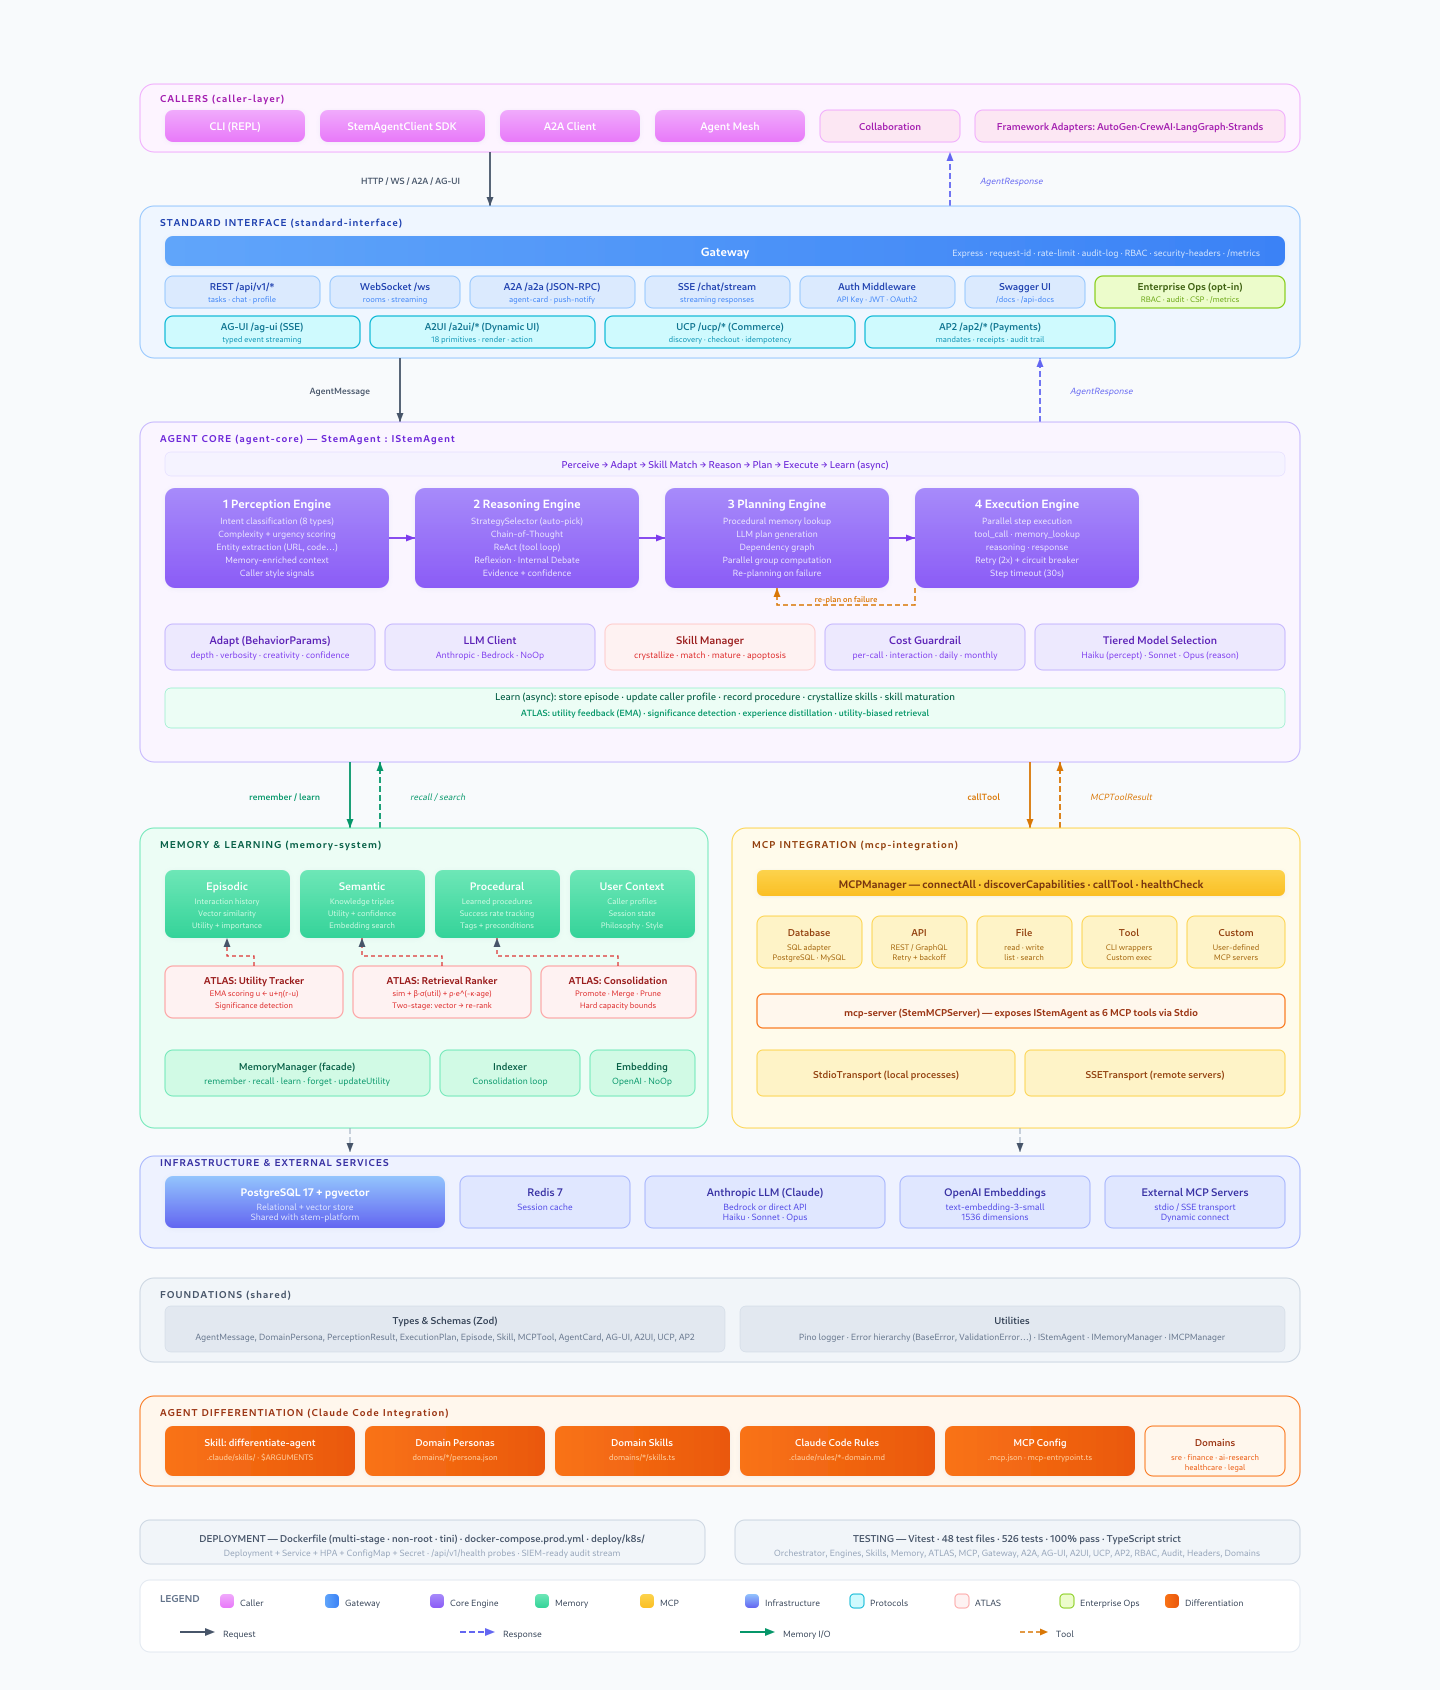
\includegraphics[width=0.62\textwidth,keepaspectratio]{architecture.png}
  \caption{STEM Agent architecture. Callers reach the gateway, which mounts five protocol handlers (A2A, AG-UI, A2UI, UCP, AP2) sharing a common middleware stack. The Agent Core runs the eight-phase cognitive pipeline (\textsc{Perceive}, \textsc{Adapt}, \textsc{MatchSkills}, \textsc{SelectStrategy}, \textsc{Reason}, \textsc{Plan}, \textsc{Execute}, \textsc{Format}, plus an asynchronous \textsc{Learn}), consuming MCP tools and a four-type memory system mediated by ATLAS (utility tracker, retrieval ranker, consolidator). The Differentiation Layer produces domain-specific variants; the Enterprise Ops surface (deployment artifacts, RBAC, SIEM audit, metrics, PII redaction) mounts as opt-in middleware on the same gateway.}
  \label{fig:architecture}
\end{figure*}

\begin{table}[t]
  \small
  \centering
  \begin{tabular}{clc}
    \toprule
    Layer & Component & Key Count \\
    \midrule
    1 & Caller / User Layer & 4 adapters \\
    2 & Standard Interface (Gateway) & 5 protocols \\
    3 & Agent Core & 5 engines \\
    X$_{\mathrm{S}}$ & Security (cross-cutting, L2$\leftrightarrow$L3) & 4 IAM plugins \\
    4 & Memory System & 4 memory types \\
    5 & MCP Integration + Server & 2 transports \\
    X$_{\mathrm{D}}$ & Differentiation (cross-cutting) & personas/skills/rules \\
    \bottomrule
  \end{tabular}
  \caption{Five-layer architecture with two cross-cutting surfaces (denoted X$_{\mathrm{S}}$, X$_{\mathrm{D}}$). The Security surface is cross-cutting because authentication, rate limiting, and audit events fire between Gateway (L2) and Agent Core (L3) on every request; the Differentiation surface is cross-cutting because personas, skills, and rules parameterize L2, L3, L4, and L5 simultaneously rather than occupying a single layer.}
  \label{tab:layers}
\end{table}

\paragraph{Cognitive pipeline.}
Each request flows through eight phases: \textsc{Perceive} (intent into 10 categories, complexity into three levels, entities, sentiment, urgency); \textsc{Adapt} (load caller profile, adjust behavior parameters); \textsc{MatchSkills} (short-circuit if a committed or mature skill fires); \textsc{SelectStrategy} and \textsc{Reason} (selector in Table~\ref{tab:strategy}, with ReAct~\citep{yao2023react}, Reflexion~\citep{shinn2023reflexion}, Internal Debate~\citep{du2023debate}, and Chain-of-Thought~\citep{wei2022chain}); \textsc{Plan} (MCP tool selection with parallel steps); \textsc{Execute} (retries with default 2, circuit breaker at 3 consecutive failures); \textsc{Format}; and an asynchronous \textsc{Learn} phase that updates the profile, records skill outcomes, and attempts crystallization.

\begin{table}[t]
  \small
  \centering
  \begin{tabular}{ll}
    \toprule
    Condition & Strategy \\
    \midrule
    Tool-requiring request          & ReAct \\
    Complexity $> 0.8$              & Reflexion \\
    Analysis or creative request    & Internal Debate \\
    Otherwise                       & Chain-of-Thought \\
    \bottomrule
  \end{tabular}
  \caption{Deterministic strategy selector used by \textsc{SelectStrategy}. The complexity threshold ($> 0.8$) and rule ordering are operational defaults derived from the internal test-suite distribution (where complexity clusters bimodally around $0.3$ and $0.85$), not from a held-out benchmark; deployers targeting a distribution with a different complexity profile should re-calibrate.}
  \label{tab:strategy}
\end{table}

\paragraph{Implementation.}
The system is a TypeScript monorepo with six workspace packages covering shared schemas (154+ Zod types), agent core, the gateway and handlers, MCP client and server layers, memory, and caller utilities. The gateway runs on Express.js~5 and mounts each protocol handler via a uniform \texttt{createRouter()} method, so that adding a new protocol affects only the handler and one line in the gateway. Authentication, rate limiting, request correlation, and structured logging are shared middleware.

\section{Protocol Gateway}
\label{sec:protocols}

The single most load-bearing design decision in STEM Agent is that all five protocols share one process and one cognitive pipeline. Table~\ref{tab:protocols} summarizes them.

\begin{table*}[t]
  \small
  \centering
  \begin{tabular}{llllp{5.5cm}}
    \toprule
    Protocol & Endpoint & Transport & Role & Use case \\
    \midrule
    A2A  & \texttt{POST /a2a}          & JSON-RPC 2.0 & External$^{\ast}$ & Agent-to-agent task delegation, messaging, agent-card discovery \\
    AG-UI & \texttt{POST /ag-ui}        & SSE           & External$^{\dagger}$ & UI streaming; maps pipeline phases to typed events \\
    A2UI & \texttt{POST /a2ui/*}       & SSE + REST    & External$^{\S}$ & Dynamic UI composition with 16 component primitives \\
    UCP  & \texttt{POST /ucp/*}        & REST          & Internal$^{\ddagger}$ & Commerce checkout sessions with idempotency \\
    AP2  & \texttt{POST /ap2/*}        & REST          & Internal$^{\ddagger}$ & Mandate-based payments with audit trail \\
    \bottomrule
  \end{tabular}
  \caption{Protocols behind the unified gateway. $^{\ast}$A2A implements the Linux Foundation A2A v0.3.0 published specification. $^{\dagger}$AG-UI follows the published AG-UI streaming event model. $^{\S}$A2UI extends a community draft of the A2UI UI-composition protocol (not a ratified standard). $^{\ddagger}$UCP and AP2 are internal protocols designed to fill commerce gaps we encountered; they have not undergone external security review or formal threat modeling and are presented as illustrative design points rather than proposed standards. Deployers should treat UCP/AP2 as first-draft protocols and add domain-specific controls.}
  \label{tab:protocols}
\end{table*}

\paragraph{External protocols.} A2A implements the Linux Foundation v0.3.0 spec over JSON-RPC 2.0 (\texttt{tasks/send}, \texttt{sendSubscribe} via SSE, \texttt{get}, \texttt{cancel}); agent cards are served at \texttt{/.well-known/agent.json}. AG-UI streams cognitive-pipeline events (\texttt{TEXT\_MESSAGE\_START}, \texttt{REASONING\_MESSAGE}, \texttt{TOOL\_CALL\_START}, \texttt{STATE\_SNAPSHOT}, \texttt{RUN\_FINISHED}) over SSE. A2UI extends a community draft with a flat adjacency-list UI model and 16 primitives (text, button, card, list, input, toggle, $\ldots$) so the agent can assemble layouts without a fixed widget hierarchy; divergence from the draft is flagged in release notes.

\paragraph{UCP (Unified Commerce Protocol, internal).} UCP is an internal protocol that formalizes a checkout-session lifecycle---create, retrieve, complete---under mandatory idempotency headers (\texttt{Idempotency-Key}, \texttt{Request-Id}, \texttt{UCP-Agent}). An idempotency cache prevents duplicate session creation when a caller retries. We designed UCP because we could not find an open commerce-checkout protocol that treated the agent, rather than a browser, as the primary client; we present it as an illustrative design point rather than a proposed standard, and it has not undergone formal security review.

\paragraph{AP2 (Agent Payments Protocol, internal).} AP2 is an internal protocol that implements a three-phase payment lifecycle: Intent Mandate $\rightarrow$ Payment Mandate $\rightarrow$ Payment Receipt. Payments below a configurable threshold can auto-approve; all transitions are appended to a per-intent audit trail. AP2 is the counterpart to UCP for authorization and is explicitly designed around mandate semantics appropriate to autonomous agents. Like UCP, AP2 has not undergone external threat modeling; we treat it as a first-draft internal design and document formal threat modeling as follow-up work.

\paragraph{Integration lessons.} Enforcing \texttt{createRouter()} uniformity, even when a protocol seems to ``want'' global state, reduced cross-protocol bugs to near zero when we added AP2 after the other four. Idempotency was the actual hard part: UCP's header contract and AP2's mandate IDs each took more review cycles than the happy-path code.

\section{Caller Profiler and Behavior Parameters}
\label{sec:profiler}

Static user models produce either bland responses or hand-tuned personas that drift. STEM Agent continuously learns a Caller Profile across four categories, building on a long line of user-modeling and generative-agent work~\citep{park2023generative}: \emph{philosophy} (8 dimensions), \emph{principles} (4), \emph{style} (5), and \emph{habits} (4), for a total of 21.\footnote{The 21 dimensions are: \textit{philosophy}---pragmatism vs.\ idealism, simplicity vs.\ completeness, risk tolerance, innovation orientation, depth vs.\ breadth, theory vs.\ practice, autonomy preference, stated values; \textit{principles}---correctness vs.\ speed, documentation importance, testing emphasis, security-mindedness; \textit{style}---formality, verbosity, technical depth, examples preference, structure preference; \textit{habits}---typical session length, iteration tendency, peak hours, common topics.}

\paragraph{EMA update.} Each dimension is updated with an exponential moving average $v_{t+1} = (1-\alpha)\,v_t + \alpha\,s_t$ at learning rate $\alpha{=}0.1$. Preliminary testing showed larger values caused profile oscillation on outlier signals and smaller values felt sluggish before tracking genuine preference shifts. Per-caller locks prevent concurrent-update conflicts.

\paragraph{Confidence gating.} Profile confidence ramps with interaction count as $\text{conf}(n) = 1 - \exp(-0.1\,n)$, reaching $\approx 0.39$ at $n{=}5$, $\approx 0.63$ at $n{=}10$, and $\approx 0.86$ at $n{=}20$. We gate on $n$ rather than on the confidence value itself because the count is observable and auditable without exposing the profile; the $n{=}5$ floor is chosen so a handful of early interactions cannot dominate the profile before the EMA has had room to average out idiosyncratic first-message signals. Below the floor the system prefers current-message signals; beyond it, profile and signal are blended by confidence weight.

\paragraph{Self-tunable behavior.} Ten parameters are adjusted during \textsc{Adapt}: reasoning depth (3), exploration (0.3), verbosity (0.5), confidence threshold (0.7), tool-use preference (0.5), creativity (0.5), proactive suggestion (on), self-reflection frequency (every 5 steps), max plan steps (10), memory retrieval breadth (10). They feed the strategy selector and planning budget, so ``how hard to think'' depends on both task and caller.

\section{Differentiation: Skills and MCP-Native Tools}
\label{sec:skills}

\paragraph{Skill lifecycle.} A skill bundles a trigger (intent patterns, domain tags, entity types), an action sequence, and maturity metadata. During \textsc{Learn}, recent episodes are grouped by action pattern; if $\geq 3$ episodes share a common action key and their topic keywords overlap in at least half the group, a \emph{progenitor} skill is created. After $k_c{=}3$ successful activations with success rate $\geq 0.6$ a skill becomes \emph{committed} and may short-circuit \textsc{Reason}$\to$\textsc{Plan}; after $k_m{=}10$ it becomes \emph{mature} and receives matching priority. Skills whose success rate falls below $0.3$ after $\geq 10$ activations undergo \emph{apoptosis} and are removed. These thresholds are operating points tuned against the existing test suite rather than against a benchmark distribution. As a concrete example, a \texttt{repo\_grep\_then\_summarize} skill crystallized in the internal-search deployment after 4 episodes chaining an MCP code-search call with a summarization step; it reached committed status after 6 additional successful activations. The mechanism is \emph{intended} to remove one LLM round-trip (the \textsc{Reason} call) from matching requests, which would reduce p50 latency by the duration of that call; we have not yet run a controlled A/B comparison against the non-short-circuited path, so we report the short-circuit as an architectural property rather than a measured speed-up.

\paragraph{From knowledge to intelligence: the Skills Manager.} Skills sit at the top of a four-step promotion ladder---episodic memory $\to$ semantic triples $\to$ procedural patterns $\to$ committed/mature skills---managed by a Skills Manager that converts outputs of the ATLAS memory subsystem (\S\ref{sec:memory}) into actionable capability. The manager consumes procedural patterns from ATLAS consolidation and cross-checks them against semantic triples above a confidence threshold; a procedure that is both empirically successful (success rate $\geq 0.6$ over $\geq k_c$ activations) and semantically coherent (stable, non-contradictory triples) is promoted to \emph{committed}. Mature skills thus represent accumulated \emph{intelligence}---reusable capability that reduces pipeline work---distinct from stored knowledge. The manager also drives apoptosis and re-promotion, and \texttt{stem\_list\_skills} exposes current capabilities for audit.

\paragraph{MCP-native tools.} All domain capabilities are acquired at runtime through MCP: database access, API integrations, file operations, and vertical tools are discovered and invoked without recompiling the agent. Meta-reasoning rules (strategy selection, parameter tuning, skill lifecycle) deliberately remain in code, not in MCP, because they are properties of the agent, not the domain.

\paragraph{Development-time differentiation.} A Domain Persona schema (\texttt{systemPrompt}, \texttt{preferredStrategy}, \texttt{defaultBehavior} overrides, \texttt{toolAllowlist}, \texttt{requiredMCPServers}, \texttt{forbiddenTopics}, \texttt{domainTags}) parameterizes the generic agent. Each domain directory holds the persona, plugin skills at committed maturity, and glob-scoped tooling rules. An \texttt{mcp-server} package wraps the running agent as MCP tools (\texttt{stem\_process}, \texttt{stem\_list\_skills}, \texttt{stem\_recall\_memory}, etc.) so other MCP clients can invoke a differentiated variant. A slash-command skill (\texttt{/differentiate-agent \$DOMAIN}) assembles and verifies all of the above. In the authors' experience, creating a new domain variant via \texttt{/differentiate-agent} appears to take on the order of minutes, compared with the multi-day effort previously required to fork and rewire an agent codebase; we do not have a controlled measurement.

\paragraph{Regulated-domain personas.} Two of the five personas target regulated verticals, showing how the \texttt{forbiddenTopics}/\texttt{toolAllowlist} contract is used for compliance (Table~\ref{tab:domains}). \emph{Healthcare} forbids direct patient diagnosis, PHI disclosure without authorization, and off-label advice; it requires MCP servers for literature, drug interactions, and an FHIR bridge, and ships a committed \texttt{phi\_redaction\_precheck} skill that runs before any external call. \emph{Legal} forbids issuing legal advice, privileged-communication disclosure, and cross-jurisdiction conclusions; its skills (\texttt{clause\_extraction}, \texttt{risk\_flagging}, \texttt{obligation\_summary}) produce review artifacts rather than final answers. These boundaries are enforced by the same guardrail path as non-regulated personas, so adding a regulated variant reduces to writing the persona JSON and skill triggers. All five templates have been exercised only within the authors' organization; we are not aware of external adopters, and the regulated personas have not been audited by compliance counsel---they encode the mechanism, not a certification.

\begin{table}[t]
  \small
  \centering
  \begin{tabular}{lll}
    \toprule
    Persona & Regulated & Representative forbidden topic \\
    \midrule
    SRE           & --- & unreviewed prod mutations \\
    Finance       & --- & personalized investment advice \\
    AI research   & --- & fabricated citations \\
    Healthcare    & HIPAA-style & PHI disclosure without authz. \\
    Legal         & attorney-client & issuing legal advice \\
    \bottomrule
  \end{tabular}
  \caption{Shipped industry personas. ``Regulated'' flags personas whose \texttt{forbiddenTopics} encode compliance boundaries; the enforcement path is identical across regulated and non-regulated personas.}
  \label{tab:domains}
\end{table}

\section{Memory System}
\label{sec:memory}

Four memory types, informed by recent agent-memory work~\citep{ai2025memorybench, gallego2026memoryastool, yadav2026synapse}, sit behind a Memory Manager facade:

\begin{itemize}
\item \textbf{Episodic.} Interaction episodes with vector embeddings and importance scores (PostgreSQL + pgvector).
\item \textbf{Semantic.} Knowledge triples (subject, predicate, object) in a concept graph, populated by pattern extraction from episodic memory.
\item \textbf{Procedural.} Successful strategies and tool-usage patterns used to prime planning on recurring tasks.
\item \textbf{User context.} Per-caller profile and session history, with an explicit forget-me path for regulatory compliance.
\end{itemize}

Consolidation moves information episodic$\to$semantic and episodic$\to$procedural as history grows; low-utility entries are pruned under capacity bounds. Together with semantic-store deduplication, this is designed for sub-linear growth under sustained interaction (exact characteristics left to future measurement).

\paragraph{ATLAS: utility-guided retrieval and consolidation.} The four tiers are mediated by ATLAS (Adaptive Tiered Learning And Storage). A \emph{utility tracker} maintains per-item EMA scores $u_{t+1} = u_t + \eta(r_t - u_t)$ driven by downstream outcome feedback (whether an item was used, whether execution succeeded, whether the caller accepted the answer); a significance detector flags high-impact items for promotion. A two-stage \emph{retrieval ranker} fetches candidates by vector similarity then re-ranks with $\mathrm{sim} + \beta\,\sigma(u) + \rho\,e^{-\kappa\,\mathrm{age}}$, where $\eta{=}0.1$ is the tracker learning rate and $\beta{=}0.3$, $\rho{=}0.2$, $\kappa{=}1/30\mathrm{d}$ weight utility and recency (defaults). A \emph{consolidator} runs promote/merge/prune passes under hard capacity bounds, guaranteeing the episodic tier cannot grow unboundedly.

\paragraph{From memory to knowledge: extraction pipeline.} The consolidation pass also turns raw interaction into structured knowledge. Episodes crossing the significance threshold with stable entity/relation patterns are distilled into semantic triples $(\textit{s}, \textit{p}, \textit{o})$ whose confidence is seeded from episode utility and updated under supporting or contradicting evidence; sub-floor or duplicate triples are retired. The same pass surfaces repeated tool-use procedures into the procedural tier. The net effect is that semantic and procedural stores grow with \emph{what has been useful}, not raw interaction volume---the property the Skills Manager relies on.

\section{Deployment Experience}
\label{sec:deployment}

STEM Agent has been deployed internally for six months, serving four production use cases (customer support, internal search, code assistance, documentation QA) to $\sim$200 weekly active users across three engineering teams. These four production configurations are distinct from the five industry-aligned persona templates shipped in the repository (SRE, finance, AI research, healthcare, legal), which are reference artifacts illustrating the differentiation mechanism across regulated and non-regulated verticals. This section reports operational lessons, scalability, and integration patterns from that period.

\paragraph{Enterprise Ops as a first-class surface.} We treat deployment artifacts, security hardening, and observability as a single \emph{Enterprise Ops} surface mounted on the same gateway as the protocol handlers. It bundles (i)~production deployment artifacts, (ii)~the opt-in hardening controls summarized in Table~\ref{tab:hardening}, and (iii)~the observability stack (correlation IDs, OpenTelemetry-compatible spans, Prometheus counters/histograms). A uniform enable/disable contract let every enterprise-review concern we encountered be resolved by wiring a middleware rather than by branching the cognitive pipeline.

\paragraph{Deployment context.} The gateway runs as a containerized service on Kubernetes (HPA 2--8 replicas, CPU-based). PostgreSQL+pgvector handles episodic memory; Redis provides idempotency and session state. Daily volume is 2,400 interactions (p50 1.2\,s, p95 3.8\,s, p99 7.1\,s). Over six months we saw 14 operator incidents (LLM rate-limit exhaustion $\times$6, MCP tool timeout $\times$4, idempotency-cache races $\times$2); mean time to resolution was 18 minutes, mostly driven by LLM-provider recovery.

\paragraph{Production deployment artifacts.} The system ships with artifacts that correspond one-to-one with the architecture: a multi-stage \texttt{Dockerfile} producing a non-root \texttt{node:22-slim} image (\texttt{tini} PID-1, \texttt{HEALTHCHECK} on \texttt{/api/v1/health}), a \texttt{docker-compose.prod.yml} overlay that externalizes \texttt{DATABASE\_URL}/\texttt{REDIS\_URL}, and a \texttt{deploy/k8s/} directory with illustrative Deployment (2 replicas, resource limits, readiness/liveness probes, non-root \texttt{securityContext}, \texttt{readOnlyRootFilesystem}), Service, ConfigMap, Secret template, and HPA manifests. These ship as \emph{example} manifests with a banner directing operators to adapt them; \texttt{docs/deployment.md} enumerates scaling caveats (in-memory rate-limiter, in-memory AP2 mandate store) and flags Redis-backed replacements as follow-ups.

\paragraph{Scalability architecture.} The cognitive pipeline is stateless between requests; all persistent state flows through the Memory Manager facade. We externalized the idempotency cache and audit trail to Redis (Lua-scripted atomic operations), eliminating the single-process constraint, and validated linear scaling to 500 concurrent requests across 8 replicas before LLM-provider rate limits became the bottleneck. The Differentiation Layer is mounted from a ConfigMap, enabling domain-variant updates without rebuilds.

\paragraph{Security and authentication.} The IAM layer is plugin-based with four providers (JWT, OAuth2, SAML, API-Key) implementing a common \texttt{IAuthenticator} with TTL-cached policy decisions. Rate limiting is per-caller; commerce protocols enforce stricter limits (10 req/min vs.\ 100 for A2A). Over six months the IAM layer blocked 47 unauthorized attempts without false positives. Auth logic is isolated from agent reasoning: adding a provider requires zero changes to the cognitive pipeline.

\paragraph{Opt-in enterprise hardening surface.} Internal security reviews repeatedly surfaced a tension: every added default risked breaking existing consumers, while every missing default drew a finding. We resolved this by making each enterprise control a separate, env-gated middleware that defaults off (Table~\ref{tab:hardening}). Authorization uses \texttt{requirePermission(perm)} factories that consume \texttt{Principal.permissions}; a SIEM-ready audit stream emits one JSON event per request---\texttt{\{ts, requestId, principal, action, resource, decision, status, latencyMs, ip\}}---via a pino child logger tagged \texttt{name:"audit"}, so downstream pipelines (fluent-bit $\to$ S3/Splunk) filter by logger name. Response-side headers (strict CSP, XFO, HSTS, Referrer-Policy; removed X-Powered-By) are a single hand-rolled middleware with no new dependency; logging ships with a default \texttt{redact} list for secrets that can be disabled via \texttt{LOG\_REDACT}. A dependency-free Prometheus exposition mounts at \texttt{/metrics} when enabled. Every control is covered by tests asserting both the enabled and disabled paths, mechanically verifying the ``defaults unchanged'' invariant.

\begin{table}[t]
  \footnotesize
  \centering
  \setlength{\tabcolsep}{3pt}
  \begin{tabular}{lll}
    \toprule
    Concern & Control & Enable via \\
    \midrule
    Headers       & CSP/HSTS/XFO mw.      & \texttt{SECURITY\_HELMET} \\
    RBAC          & \texttt{requirePermission} & per-route \\
    Audit stream  & pino (\texttt{audit}) child  & \texttt{AUDIT\_LOG\_ENABLED} \\
    PII redact    & pino \texttt{redact}     & on; \texttt{LOG\_REDACT=off} \\
    Metrics       & Prom.\ \texttt{/metrics} & \texttt{METRICS\_ENABLED} \\
    \bottomrule
  \end{tabular}
  \caption{Opt-in hardening controls. All default off except PII redaction (on by default; secret leakage is strictly worse than quickstart friction). Enabling requires no gateway/handler code changes.}
  \label{tab:hardening}
\end{table}

\paragraph{Observability and tracing.} Every request is assigned a correlation ID that propagates through all eight pipeline phases; logs are JSON-formatted with consistent fields (correlation\_id, caller\_id, phase, latency\_ms, status). OpenTelemetry traces yield per-phase latency breakdowns (e.g., \textsc{Perceive} 80\,ms, \textsc{Reason} 1,100\,ms, \textsc{Execute} 200\,ms) and Prometheus metrics track request counts, latency histograms, skill activations, and MCP invocation frequencies. This stack was essential for diagnosing the idempotency race condition: traces revealed duplicate cache writes under concurrent retries, resolved by compare-and-swap semantics in Redis.

\paragraph{Test suite.} The suite comprises 535 Vitest tests across 48 files (total runtime $<$4\,s), passing at 100\% on the 47 files in this release. Coverage spans per-engine unit tests, all five protocol handlers, memory stores, MCP integration via \texttt{InMemoryTransport}, persona schema validation, IAM middleware, and the enterprise-hardening middleware (RBAC allow/deny, audit \texttt{decision} fields, security-header presence). Hardening tests assert both the enabled and disabled paths so opt-in gating cannot silently regress.

\paragraph{Integration patterns.} Four framework adapters (AutoGen, CrewAI, LangGraph, OpenAI Agents SDK) translate external conventions to the internal message format, letting teams call STEM Agent as an A2A peer without rewriting callsites. A CrewAI-based customer-support bot was migrated in about two hours by swapping tool invocations for A2A delegate calls. The repository also ships an \emph{enterprise-ops smoke test}: a single executable example that walks a deployer through an authenticated call (\texttt{X-API-Key}), a request-id correlation pivot, an RBAC-gated endpoint probe, and a \texttt{/metrics} scrape; it degrades gracefully when auth or metrics are disabled.

\paragraph{Feature comparison.} Table~\ref{tab:comparison} contrasts the STEM surface with prior systems by whether each framework ships a named subsystem for the capability. Protocol counts reflect published externally-maintained specifications.

\begin{table}[t]
  \footnotesize
  \centering
  \setlength{\tabcolsep}{3pt}
  \begin{tabular}{lccccc}
    \toprule
    Framework & Proto. & Adapt & Mem. & Skills & Com. \\
    \midrule
    AutoGen~\citep{wu2023autogen}        & 1 & \texttimes & \checkmark & \texttimes & \texttimes \\
    MetaGPT~\citep{hong2023metagpt}      & 1 & \texttimes & \checkmark & \texttimes & \texttimes \\
    CrewAI~\citep{crewai2023}            & 1 & \texttimes & \checkmark & \texttimes & \texttimes \\
    LangChain~\citep{chase2022langchain} & 1 & \texttimes & \checkmark & \texttimes & \texttimes \\
    \textbf{STEM} & \textbf{5\,(3+2$^\dagger$)} & \checkmark & \textbf{4} & \checkmark & \checkmark \\
    \bottomrule
  \end{tabular}
  \caption{Capability-surface comparison. Proto.\ = interoperability protocols; Adapt = per-caller adaptation subsystem; Mem.\ = named memory subsystem or type count; Skills = emergent skills; Com.\ = commerce. $\dagger$UCP/AP2 are internal first-draft (no external security review).}
  \label{tab:comparison}
\end{table}

\section{Conclusion}
\label{sec:conclusion}

STEM Agent demonstrates that protocol plurality, self-adaptation, and emergent skills can coexist in a production system when domain knowledge is kept behind MCP and user modeling is decoupled from domain logic. Six months of internal deployment across four use cases ($\sim$200 weekly users) and five persona templates (two regulated) validate the approach: pluggable IAM met enterprise auth without touching agent logic, the opt-in hardening surface satisfied security review without changing the quickstart path, and the shipped Dockerfile+Kubernetes manifests reduced deployment discussions to \texttt{kubectl diff}. Ongoing work: learned strategy selection~\citep{alomrani2025reasoning}, more protocols~\citep{chang2025anp, nie2026awcp}, embedding-based skill matching, UCP/AP2 threat modeling~\citep{anbiaee2026security}, Redis-backed replacements, and wiring the OpenTelemetry SDK.

\section*{Limitations}

\textbf{No public benchmark comparison.} We report production metrics from internal deployment but do not compare task-completion scores against public multi-agent benchmarks (e.g., MAFBench~\citep{orogat2026mafbench} or MCP-Universe~\citep{luo2025mcpuniverse}). The feature-comparison table contrasts capability surfaces, not benchmark performance.

\textbf{Single-organization deployment.} All operational data comes from one enterprise context. Generalization to other domains, team structures, or traffic patterns requires external validation.

\textbf{Adaptation model simplicity.} The EMA-based Caller Profiler cannot represent non-stationary or multi-modal preference distributions, and confidence gating is a scalar rather than per-dimension signal.

\textbf{Protocol maturity.} UCP and AP2 are proposed here and have no external adoption, formal threat model, or conformance suite. Deployers should treat these as first-draft protocols and add domain-specific security controls.

\textbf{Deterministic strategy selection.} Reasoning-strategy selection uses hand-written rules rather than a learned policy and has not been tuned against a benchmark distribution.

\textbf{LLM-provider bottleneck.} Observed p99 latency (7.1\,s) is dominated by LLM inference time; our architectural optimizations target protocol overhead and state management, not model reasoning speed.

\textbf{Opt-in hardening is not a substitute for deployment-site review.} The controls in Table~\ref{tab:hardening} are audit-friendly primitives (RBAC factory, structured audit events, strict headers, PII redaction, \texttt{/metrics}), not a compliance certification. They materially reduce the work a deployer must do to stand up a reviewable baseline, but they do not replace a site-specific threat model, a penetration test, or the per-vertical controls that regulated domains require on top of the shared enforcement path.

\section*{Ethical Considerations}

The Caller Profiler stores per-user behavioral signals. To mitigate privacy and consent risks we (i)~expose a GDPR-style forget-me operation that removes all per-caller profile and session state; (ii)~keep profile updates reversible (EMA with bounded $\alpha$ so a single misclassified signal cannot dominate); (iii)~scope audit logs at the request level so misuse can be traced without exposing content. The commerce protocols (UCP, AP2) handle payment intents; in deployment we require human approval above a configurable threshold and emit a complete per-intent audit trail, but we stress that UCP/AP2 have not undergone formal security review. Any deployer should treat these as first-draft protocols and add domain-specific guardrails. More broadly, agent frameworks that integrate authentication, commerce, and persistent user modeling into one process enlarge the blast radius of a compromise; the pluggable IAM layer and layered architecture are partial mitigations, not a substitute for operational review.

\bibliography{references}

\end{document}
